\section{Holiday and Sick Leave Detection}

The information about anomalies in the regular work pattern can be a valuable information for several parties.
Usually only few parties people know about the holiday or sick leave times of a person.
To know if a persons tends to become sick often or for long times is a dangerous intrusion into a persons privacy.
For instance this could be abused by head hunters or personnel managers to cull possible employees with too high sick leave rates and thereby reduce the job prospects of the target.

For employees this might convenient to detect anomalies in the productivity of an employee.
In case an employee doesn't commit on a regular basis for several days, this behaviour would be instantly visible with this method.

Another attack vector could be to look at the correlation of miss-out between several employees.
This attack could even be performed by an outsider, if the employees of a company are known.
The information gained by this attack could be quite delicate, as they could reveal relationships between employees.
This attack is heavily inspired by an article about data mining articles from the popular German weekly magazine \emph{Der Spiegel} written by the David Kriesel~\cite{article:spiegel-mining}.


\subsection{Implementation}

The requirements for this algorithm is the detection of a regular work pattern for a given interval.
It must have the ability to adjust to a changing work pattern, but at the same time has to be capable of detecting anomalies in this pattern.
If the attacker wants to look at multiple people, some kind of measure for similarity in the missing time patterns has to exist.

The input for this analysis is the intersection between all commits from the considered repositories and all commits from the considered contributors.
The commits' meta data used for this analysis are time stamps as well as additions and deletions in lines of code.

\begin{figure}[H]
    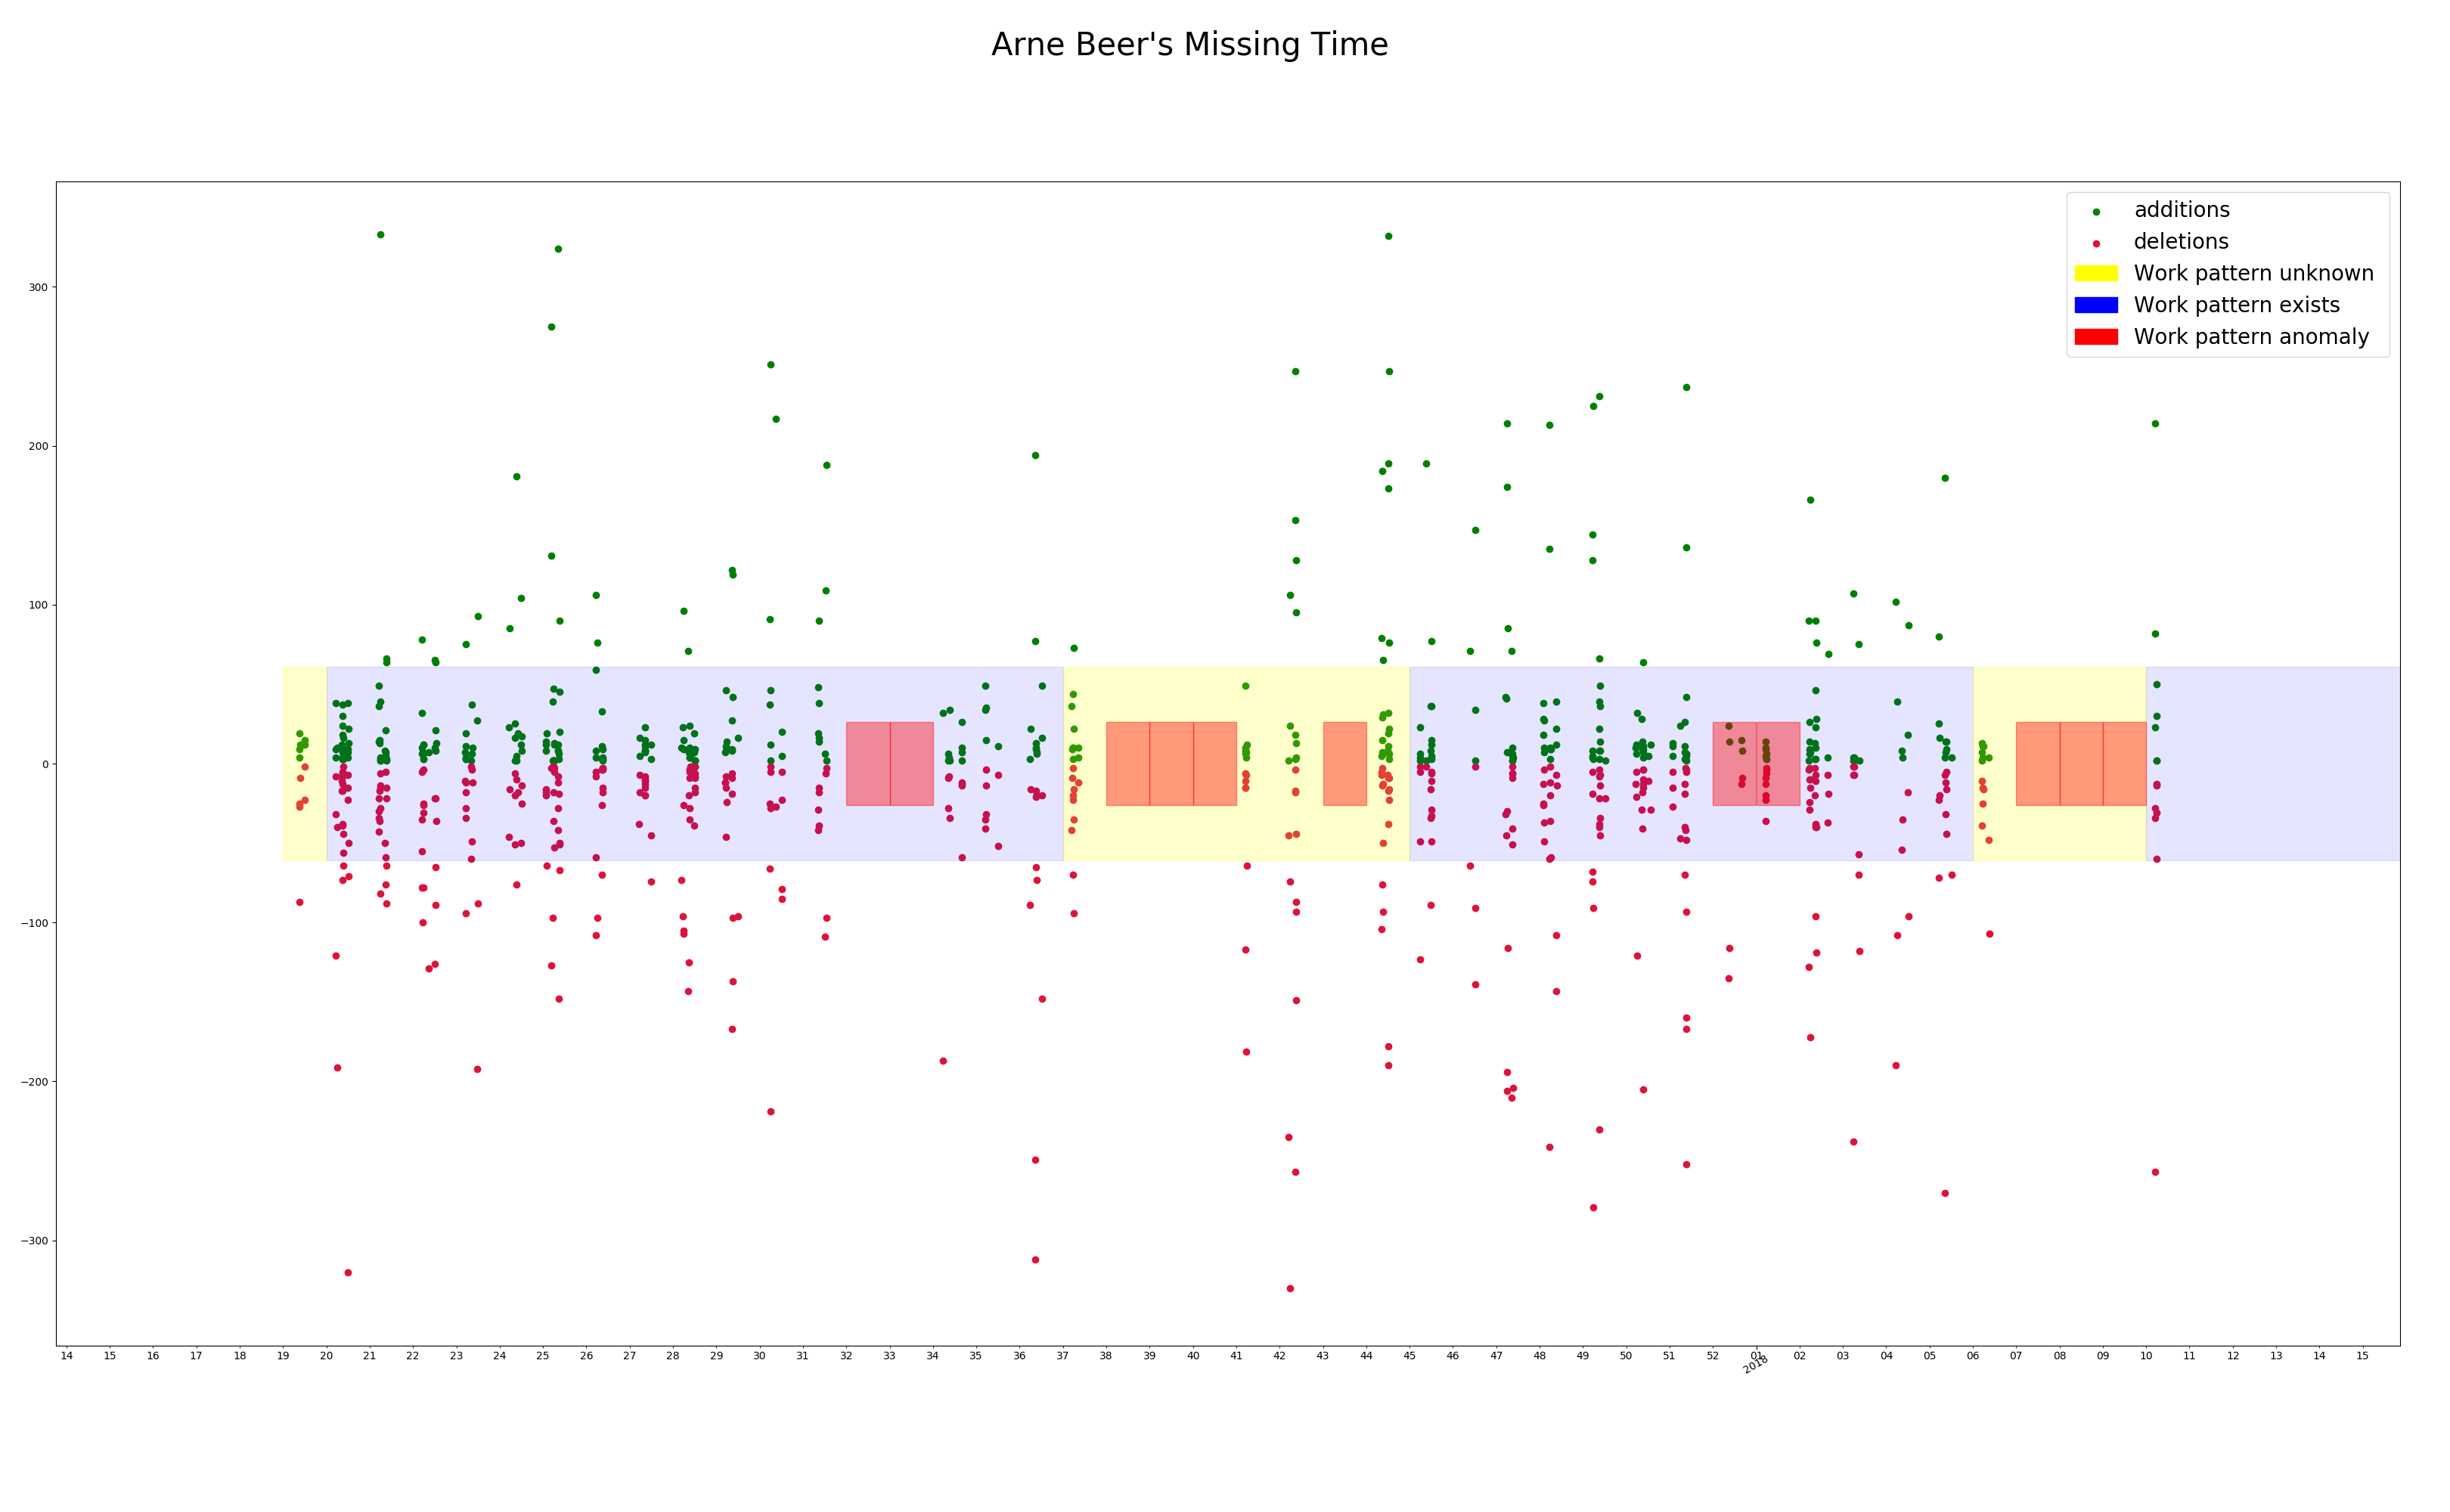
\includegraphics[scale=0.20]{./graphs/analysis/work-time-analysis}
    \centering
    \caption{The work time analysis of the author.}\label{fig:missing-time}
\end{figure}

The analysis of the data is a chronological scan of all commits for specific user.
Before performing the actual analysis, the data is converted into a usable format representing the week days.
The converted data format represents the amount of commits for each day in the last year.
It is really difficult to measure productivity in lines of code committed or in the amount of commits made by a person, as they don not necessarily display the amount of work that have been put into those commits.
As a result I decided, that a day counts as a work day as long as at least single commit has been made during the day.

\begin{minted}{python}
def analyse(weeks):
    prototype = None
    for index, week in weeks.items():
        next_six_weeks = weeks[index:index+future_lookup]
        if not prototype:
            # See if there is a prototype in the next few weeks.
            prototype = find_prototype(next_six_weeks)

            # Check if this specific week is a anomaly
            check_anomaly(prototype, week)

            continue

        prototype_exists = prototype_exists_in_next_weeks(next_six_weeks)
        if not prototype_exists:
            # We couldn't find the prototype in the next few rows
            # Try to find a new prototype
            prototype = find_prototype(next_six_weeks)

        check_anomaly(prototype, week)


def check_anomaly(prototype, week):
    if week.working_days == 0:
        save_anomaly(week)

    if prototype is not None:
        different_days = week.working_days - prototype.working_days
        // A single day variance is acceptable
        if different_days >= 1:
            save_anomaly(week)

\end{minted}
\begingroup
\captionof{listing}{Miss-out analysis \label{lst:naive-path-tracing}.}
\endgroup

The algorithm inspects every week work pattern of a given interval.
At the beginning a new \emph{prototype} is tried to be found.
A prototype is a representative week work pattern, which resembles the average work day pattern of the next weeks.
This happens in the function \inlinecode{find\_prototype}.
It performs a simple iteration over a given interval to find a work day pattern, which occurs more often than a given threshold.
If a prototype is found, we are capable of identifying anomalies that deviate from this pattern.

For each following week it is firstly checked if this week is a anomaly for this prototype.
Anomalies are simply detected by comparing the amount of working days of the prototype and the currently looked at week.
The real difference in the working pattern is not suitable for this analysis, as it produces too many false positives for employees with flexible work time.

Secondly it is checked if there exists a week in the near future, which is identical to the prototype.
If there is no week identical to the prototype in the near future, the current prototype is reset and a new prototype needs to be found.

In case no prototype can be found, anomalies cannot be easily identified, as there exists no pattern to check against.
Only obvious anomalies, namely weeks without a single work day, will then be marked as such.


\subsection{Interpretation and evaluation}

Figure~\ref{fig:missing-time} shows the analysis of the author for his work repositories.
The y-axis shows the additions or deletions per commit, the x-axis shows the week of a year.
For better analysis and evaluation of the results, a scatter plot with the additions and deletions per commit has been added on top of the miss-out graph.

The evaluation of this algorithm turned out to be quite difficult, as there is no publicly available information about sick leave or holiday.
For the purpose of this thesis I had to use anonymous statistics of several friends and colleagues to evaluate the algorithm.
The algorithm successfully manages to find all anomalies, which occurred in the last year, for all seven regarded users.

An unexpected side effect of detecting prototypes is that the algorithm also also finds inconsistencies in the work routine.
For instance between week 37 to 45 in Figure~\ref{fig:missing-time} I was forced to reduce my working hours due to legal questions and shift hours and working days.
It is hard to interpret those inconsistencies without more contextual information, but nevertheless it provides the fact that something happened during this time.

\begin{figure}[H]
    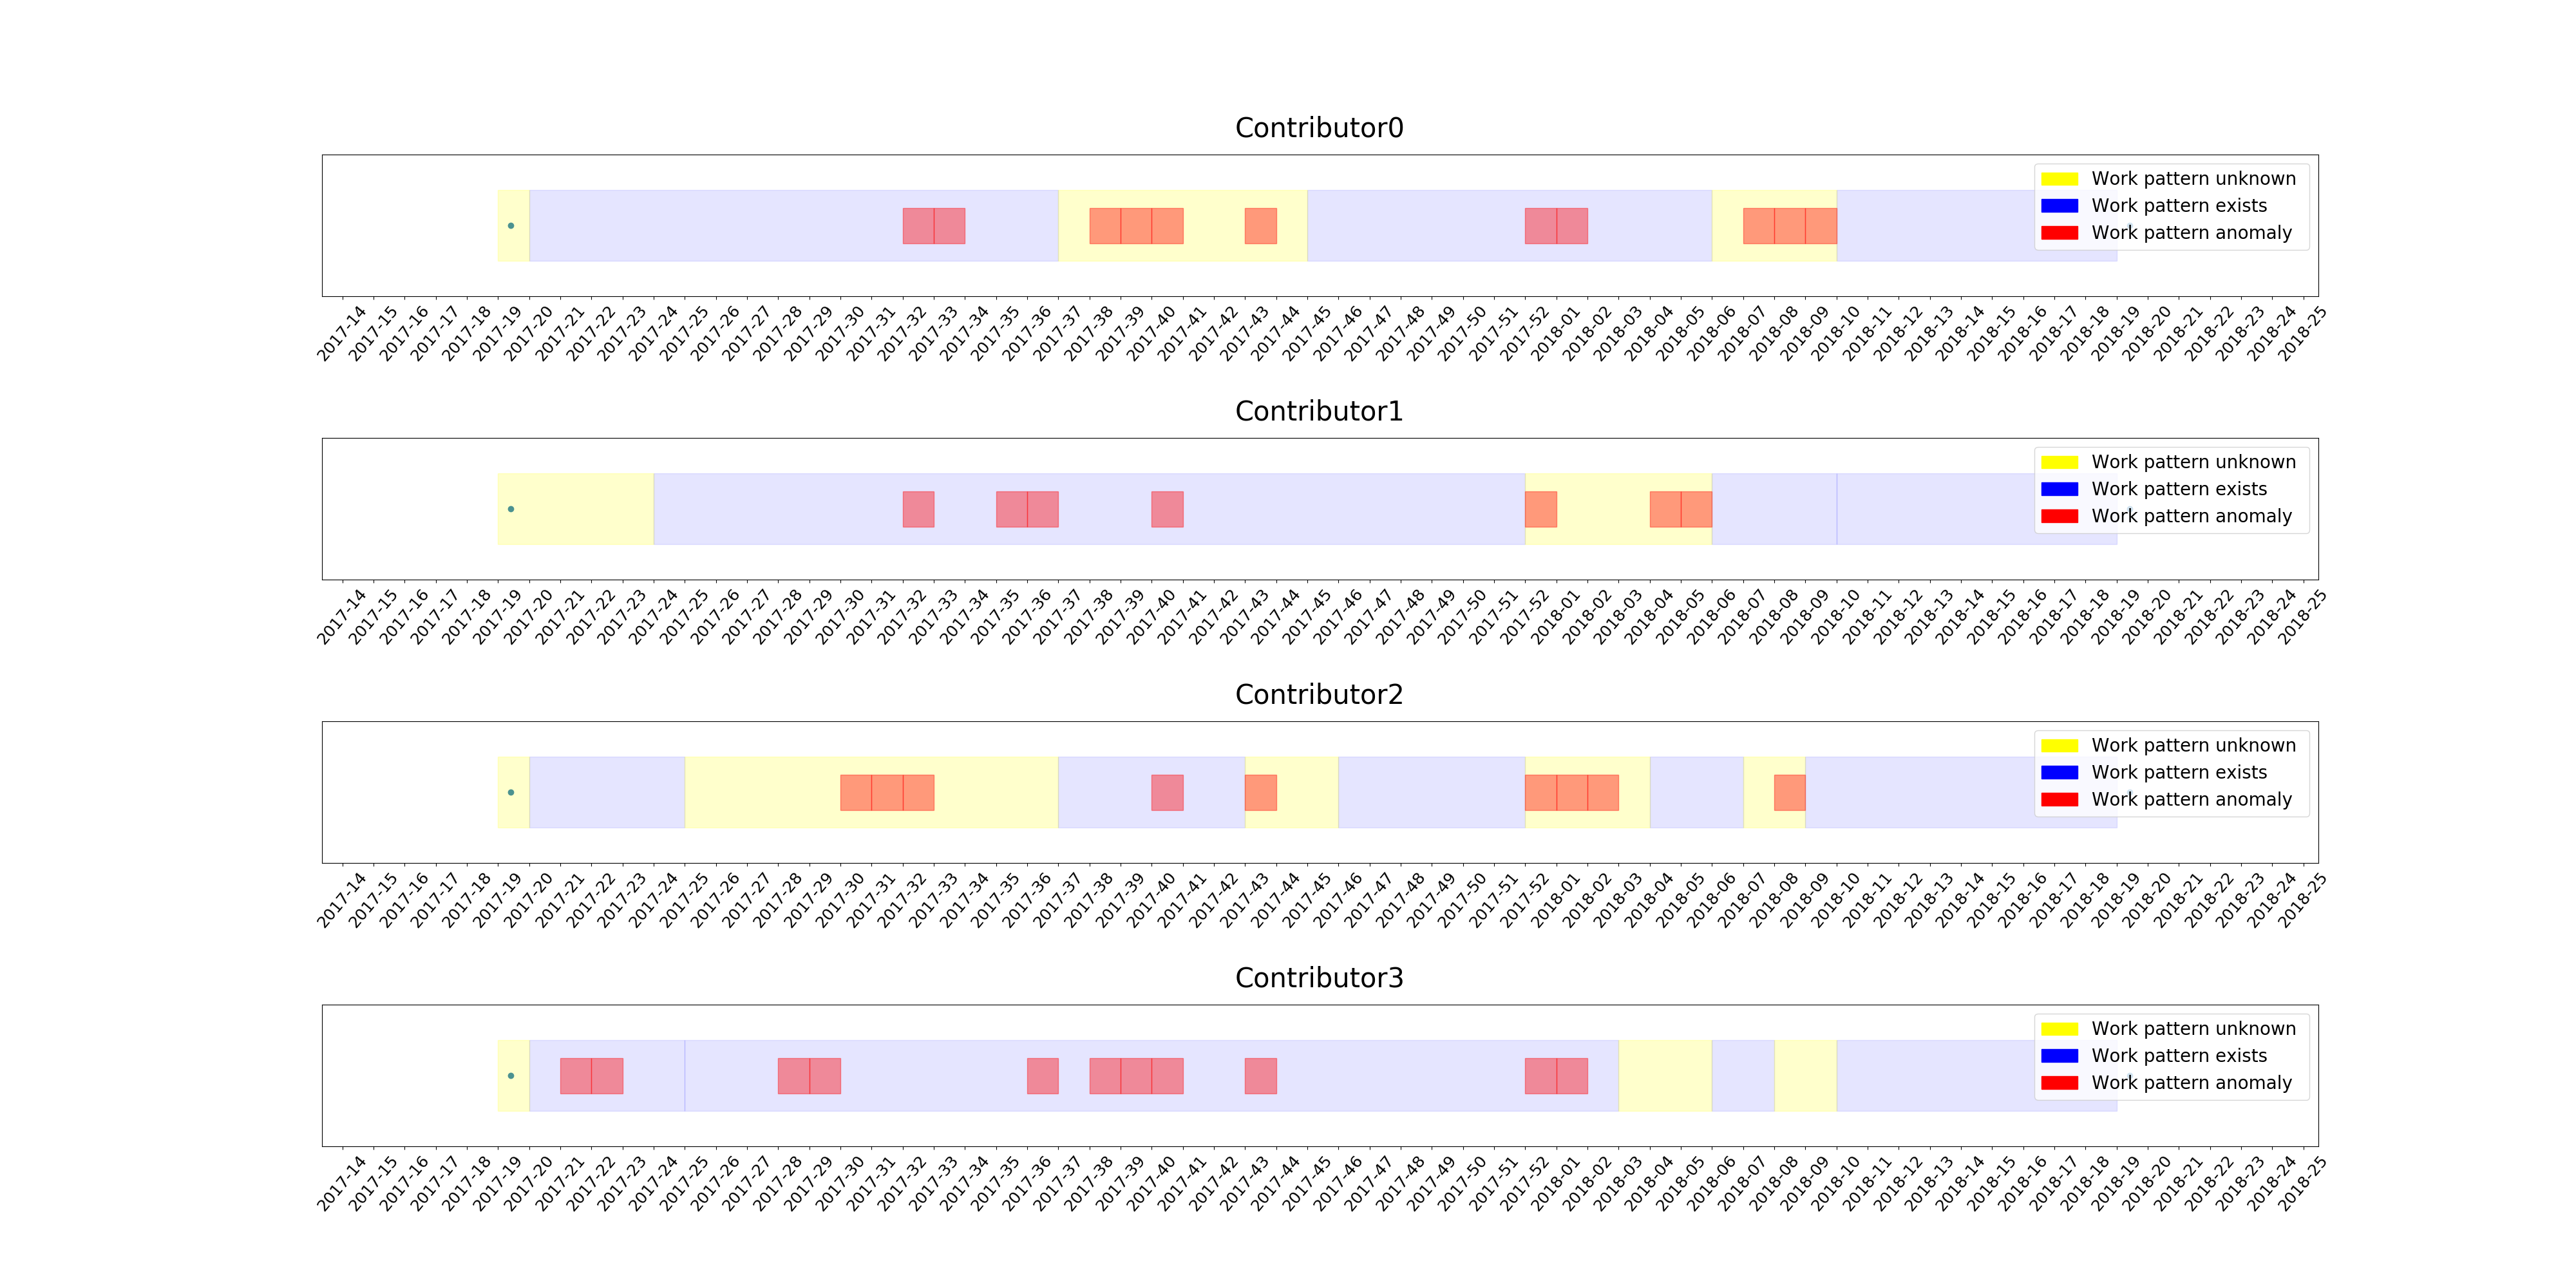
\includegraphics[scale=0.20]{./graphs/analysis/work-time-analysis-comparison}
    \centering
    \caption{The miss-out analysis of several employees.}\label{fig:miss-out-comparison}
\end{figure}

In Figure~\ref{fig:miss-out-comparison} the comparison between multiple employees can be seen.
Contributor0 and Contributor2 are working on flexible work time, while the other two contributors have regular working hours, which reflects in the inconsistencies of those contributors.
